%% This is file `elsarticle-template-1-num.tex',
%%
%% Copyright 2009 Elsevier Ltd
%%
%% This file is part of the 'Elsarticle Bundle'.
%% ---------------------------------------------
%%
%% It may be distributed under the conditions of the LaTeX Project Public
%% License, either version 1.2 of this license or (at your option) any
%% later version.  The latest version of this license is in
%%    http://www.latex-project.org/lppl.txt
%% and version 1.2 or later is part of all distributions of LaTeX
%% version 1999/12/01 or later.
%%
%% The list of all files belonging to the 'Elsarticle Bundle' is
%% given in the file `manifest.txt'.
%%
%% Template article for Elsevier's document class `elsarticle'
%% with numbered style bibliographic references
%%
%% $Id: elsarticle-template-1-num.tex 149 2009-10-08 05:01:15Z rishi $
%% $URL: http://lenova.river-valley.com/svn/elsbst/trunk/elsarticle-template-1-num.tex $
%%
\documentclass[preprint,12pt]{elsarticle}

%% Use the option review to obtain double line spacing
%% \documentclass[preprint,review,12pt]{elsarticle}

%% Use the options 1p,twocolumn; 3p; 3p,twocolumn; 5p; or 5p,twocolumn
%% for a journal layout:
%% \documentclass[final,1p,times]{elsarticle}
%% \documentclass[final,1p,times,twocolumn]{elsarticle}
%% \documentclass[final,3p,times]{elsarticle}
%% \documentclass[final,3p,times,twocolumn]{elsarticle}
%% \documentclass[final,5p,times]{elsarticle}
%% \documentclass[final,5p,times,twocolumn]{elsarticle}

%% if you use PostScript figures in your article
%% use the graphics package for simple commands
%% \usepackage{graphics}
%% or use the graphicx package for more complicated commands
%% \usepackage{graphicx}
%% or use the epsfig package if you prefer to use the old commands
%% \usepackage{epsfig}

%% The amssymb package provides various useful mathematical symbols
\usepackage{amssymb}
%% The amsthm package provides extended theorem environments
%% \usepackage{amsthm}

%% The lineno packages adds line numbers. Start line numbering with
%% \begin{linenumbers}, end it with \end{linenumbers}. Or switch it on
%% for the whole article with \linenumbers after \end{frontmatter}.
\usepackage{lineno}
\usepackage{hyperref}
\usepackage{float}

%% natbib.sty is loaded by default. However, natbib options can be
%% provided with \biboptions{...} command. Following options are
%% valid:

%%   round  -  round parentheses are used (default)
%%   square -  square brackets are used   [option]
%%   curly  -  curly braces are used      {option}
%%   angle  -  angle brackets are used    <option>
%%   semicolon  -  multiple citations separated by semi-colon
%%   colon  - same as semicolon, an earlier confusion
%%   comma  -  separated by comma
%%   numbers-  selects numerical citations
%%   super  -  numerical citations as superscripts
%%   sort   -  sorts multiple citations according to order in ref. list
%%   sort&compress   -  like sort, but also compresses numerical citations
%%   compress - compresses without sorting
%%
%% \biboptions{comma,round}

% \biboptions{}


\journal{GSoC KDE 2017}

\begin{document}

\begin{frontmatter}

%% Title, authors and addresses

%% use the tnoteref command within \title for footnotes;
%% use the tnotetext command for the associated footnote;
%% use the fnref command within \author or \address for footnotes;
%% use the fntext command for the associated footnote;
%% use the corref command within \author for corresponding author footnotes;
%% use the cortext command for the associated footnote;
%% use the ead command for the email address,
%% and the form \ead[url] for the home page:
%%
%% \title{Title\tnoteref{label1}}
%% \tnotetext[label1]{}
%% \author{Name\corref{cor1}\fnref{label2}}
%% \ead{email address}
%% \ead[url]{home page}
%% \fntext[label2]{}
%% \cortext[cor1]{}
%% \address{Address\fnref{label3}}
%% \fntext[label3]{}

\title{Finishing started activities for GCompris in Qt-Quick}

%% use optional labels to link authors explicitly to addresses:
%% \author[label1,label2]{<author name>}
%% \address[label1]{<address>}
%% \address[label2]{<address>}

\author{Rudra Nil Basu}

\address{ \textbf{Email ID}: rudra.nil.basu.1996@gmail.com}
\address{ \textbf{Freenode IRC Nick}: rudra}
\address{ \textbf{Location}: Kolkata, West Bengal, India UTC+5.30}
%\address{ \textbf{Mentor}: Bruno Coudoin (bruno.coudoin@gcompris.net)}
%\address{ \textbf{Co-Mentor}: Johnny Jazeix (jazeix@gmail.com), }

\end{frontmatter}

%%
%% Start line numbering here if you want
%%
%\linenumbers

%% main text
\section{Motivation}
\label{S:1}

%GCompris is about teaching the basics in the most easiest way to children between the age of 2 to 10. The gtk+ version of GCompris was very well recieved, and from there it was decided to Qt version, to make GCompris available for all kinds of devices, like tablets. The latest version of GCompris is 0.70 and as of now it has 137 categories on various topics like science, maths, games and much more, fully supporting 15 languages.

GCompris is a high-quality educational suite which aims at making learning easier for children aged 2 to 10. GCompris currently has 137 activities on various topics such as science, maths, games with which it has successfully created a great learning environment for children. However, there are few activities which were started previously but is not yet complete. I strongly believe in what GCompris stands for and in this project, I aim at taking GCompris one step forward by finishing three started activities: \textit{Pilot a Submarine}, \textit{Family} and \textit{Digital Electronics}


%As of \today , a brief statistics of GCompris are:
%\begin{itemize}
%\item Latest Version: 0.70
%\item A total of 137 categories on various topics like science, maths, games and much more.
%\item 15 languages fully supported
%\item More than 100000 downloads on the Google Play Store
%\item The new version contains 8 new activities
%\end{itemize}

%My goal for the project is to port two experimental activities from the Gtk+ version of GCompris to the Qt version.

%The best way to teach any concept is by demonstration. But it is not always possible to demonstrate everything that needs to be taught, such as the working of submarine and it's different parts. That's were simulation of real world problems come to play. The aim of this project is to simulate real world situations in two activities, \textit{"Pilot a Submarine"} and \textit{"Sea race (Single Player)"}

\section{Project Goals}
\label{S:1}

By the end of the Google Summer of Code's time period, I will be completing the following started activities :

\begin{itemize}

\item \textbf{Pilot a Submarine}: It is a port to the Qt version of a strategic activity originally present in the Gtk+ version aimed to teach how a submarine works. It was started in this branch: 

\href{https://cgit.kde.org/gcompris.git/log/?h=gsoc-submarine}{https://cgit.kde.org/gcompris.git/log/?h=gsoc-submarine}

The activity needs to be started from scratch, since not much advancement has been made in the branch

\item \textbf{Family}: It is an activity to help children understand how they are related to their relatives. It was started in the branch:

\href{https://cgit.kde.org/gcompris.git/log/?h=GSoC-family}{https://cgit.kde.org/gcompris.git/log/?h=GSoC-family}

The core implementation of this activity is complete, but improvements needs to be done on the design

\item \textbf{Digital Electronics}: This activity is aimed at providing a real time simulation of an electric circuit. It was started in the branch:

\href{https://cgit.kde.org/gcompris.git/log/?h=gsoc_pulkit_digital_electricity}{https://cgit.kde.org/gcompris.git/log/?h=gsoc-pulkit-digital-electricity}

A “Free Mode” already exists, levels and tutorials needs to be added to allow children to understand and use the components properly

\end{itemize}

% =======================
% Garbage Recycle
% =======================
%\item \textbf{Garbage Recycle}: This activity is aimed to teach garbage classification. This was started in \href{https://cgit.kde.org/gcompris.git/log/?h=SoK_Activity_recyclebin_shivansh} {recyclebin} branch

%Discussions:

%\href{https://phabricator.kde.org/T339}{https://phabricator.kde.org/T339}

% =======================
% Garbage Recycle
% =======================

%\item \textbf{The Solar System}: This activity aims at providing a basic understanding about our Solar System, it's planets and facts and properties of each of the planets.

%\textbf{Additional Task}:

%If time permits me, I will be working on one more activity which has not been started yet, but discussions were ongoing for the implementation of the activity:

%\begin{itemize}

%\item \textbf{Object Arrangement}: This activity is aimed at teaching arranging objects in a given order based on factors like height and width.

%The activities for arranging numbers and alphabets in either ascending or descending order is already in review and this will be a generic one, adding all kinds of ordering activities to the project.

%Discussions:

%\href{https://phabricator.kde.org/T1956}{https://phabricator.kde.org/T1956}
%\end{itemize}

\section{Implementation Details}
\label{S:1}

\subsection{Pilot a Submarine}

The  \textit{"Pilot a Submarine"} is to learn how a submarine works, explaining the usage of elements such as engine, rudders and air tanks, in order to navigate a submarine to a required depth. It was originally started in the \href{https://cgit.kde.org/gcompris.git/log/?h=gsoc-submarine}{gsoc-submarine} branch, but not much advancement has been made. So it needs to be started from scratch.

\textbf{Main Goals:}

\begin{itemize}

\item Since this activity was already present in the Gtk+ version, I will be using the svg and the audio files from the resources used in the Gtk+ submarines activity. This will allow me to dive into the coding part directly. 

\item I will be using box2d for the simulation and handling physics and collisions

\item There will be a tutorial at the start of the activity, which will give a brief description about the different elements (engine, rudders and air tanks) and it's functions.

\item Firstly I will be implementing the submarine and the mechanics of its elements, namely the engine, rudders and the air tanks. Once that is in place, I will start creating various levels and it's variations.

%The Gtk+ version had only 4 levels, and I will increase the number of levels in the Qt port, increasing the difficulty curve, bringing up elements like caves, rocks, while still keeping it doable for children within the prescribed age limit.

\item The aim is to make the activity easy for children to understand. For achieving this, the levels should start from the very basics. The implementation is divided into two parts: 

\begin{itemize}
\item the initial levels, which are aimed at giving a basic understanding of the use of different elements required to control a submarine. For example, the first level will explain the use of engines of a submarine and will ask the user to move from one point to the other by using the engine only. Similarly, the next levels will focus on using the ballast tanks, rudders and other elements of a submarine
\item the latter levels will use the concepts from the initial levels in various forms to check whether the child has fully understood the mechanism of controlling the submarine or not
\end{itemize}
\item The activity will contain pickups in the form of jewels, as it was present in the Gtk+ version

\item Besides the regular pickups in the Gtk+ version, there will be additional threats in the form of rocks and caves, in order to maintain an increasing difficulty curve, while still keeping it doable for children within the prescribed age limit.

\item In order to enhance the experience, the overall activity and the movement of the submarine and the animations will be smoother compared to the Gtk+ activity.

\begin{figure}[H]
\centering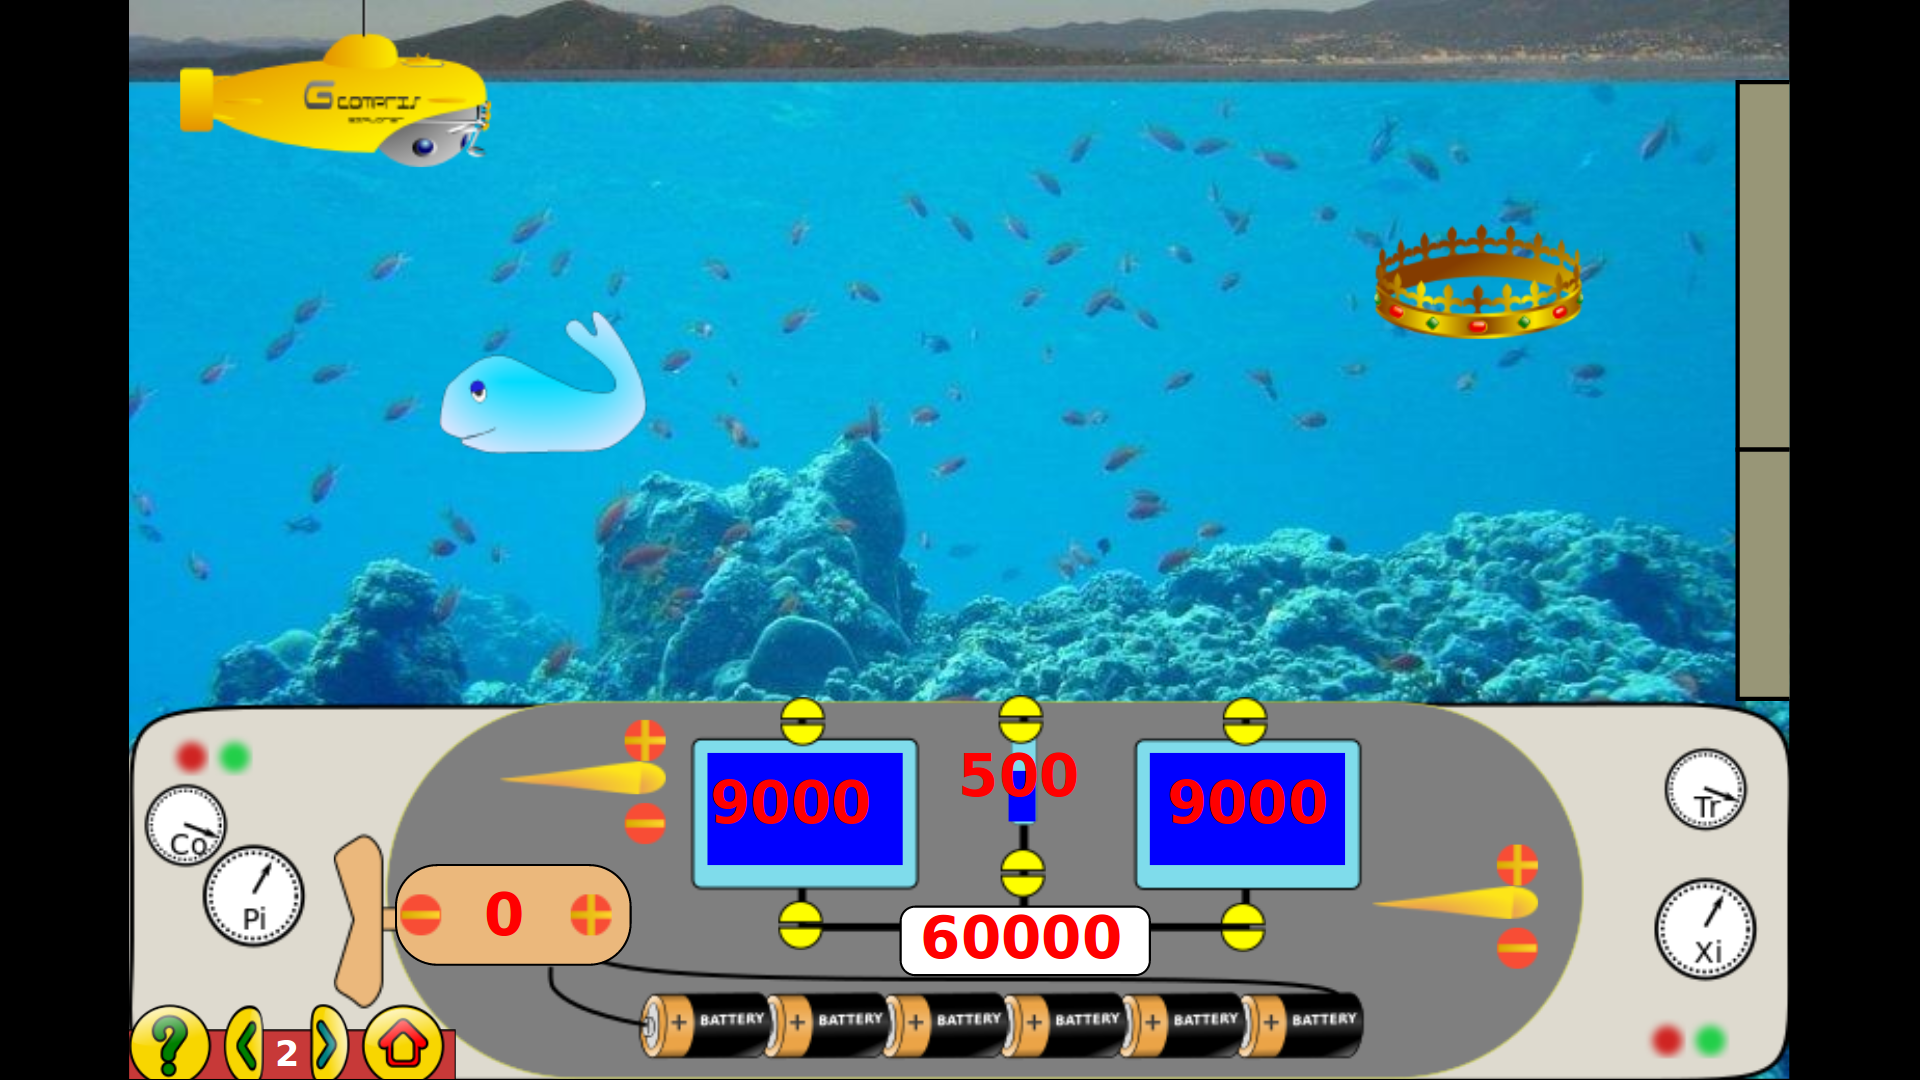
\includegraphics[width=0.9\linewidth]{submarine}
\caption{Submarine Activity}
\end{figure}

\end{itemize}

\textbf{Extended Goals:}

\begin{itemize}

\item I will look forward to improve the controls of the submarine, to make it more intuitive for the children to understand and use

\end{itemize}

\subsection{Family}

The core implementation of the family activity is finished. The layout of the activity needs to be improved.

\textbf{Main Goals:}

\begin{itemize}
\item The layout of the activity will be improved, keeping same generation members in the same level in the tree representation, making the relation easy to understand
\item Cleaning up the code: including but not limited to removing redundant variables, separating the main working code and the dataset, keeping them in different files
\end{itemize}

\begin{figure}[H]
\centering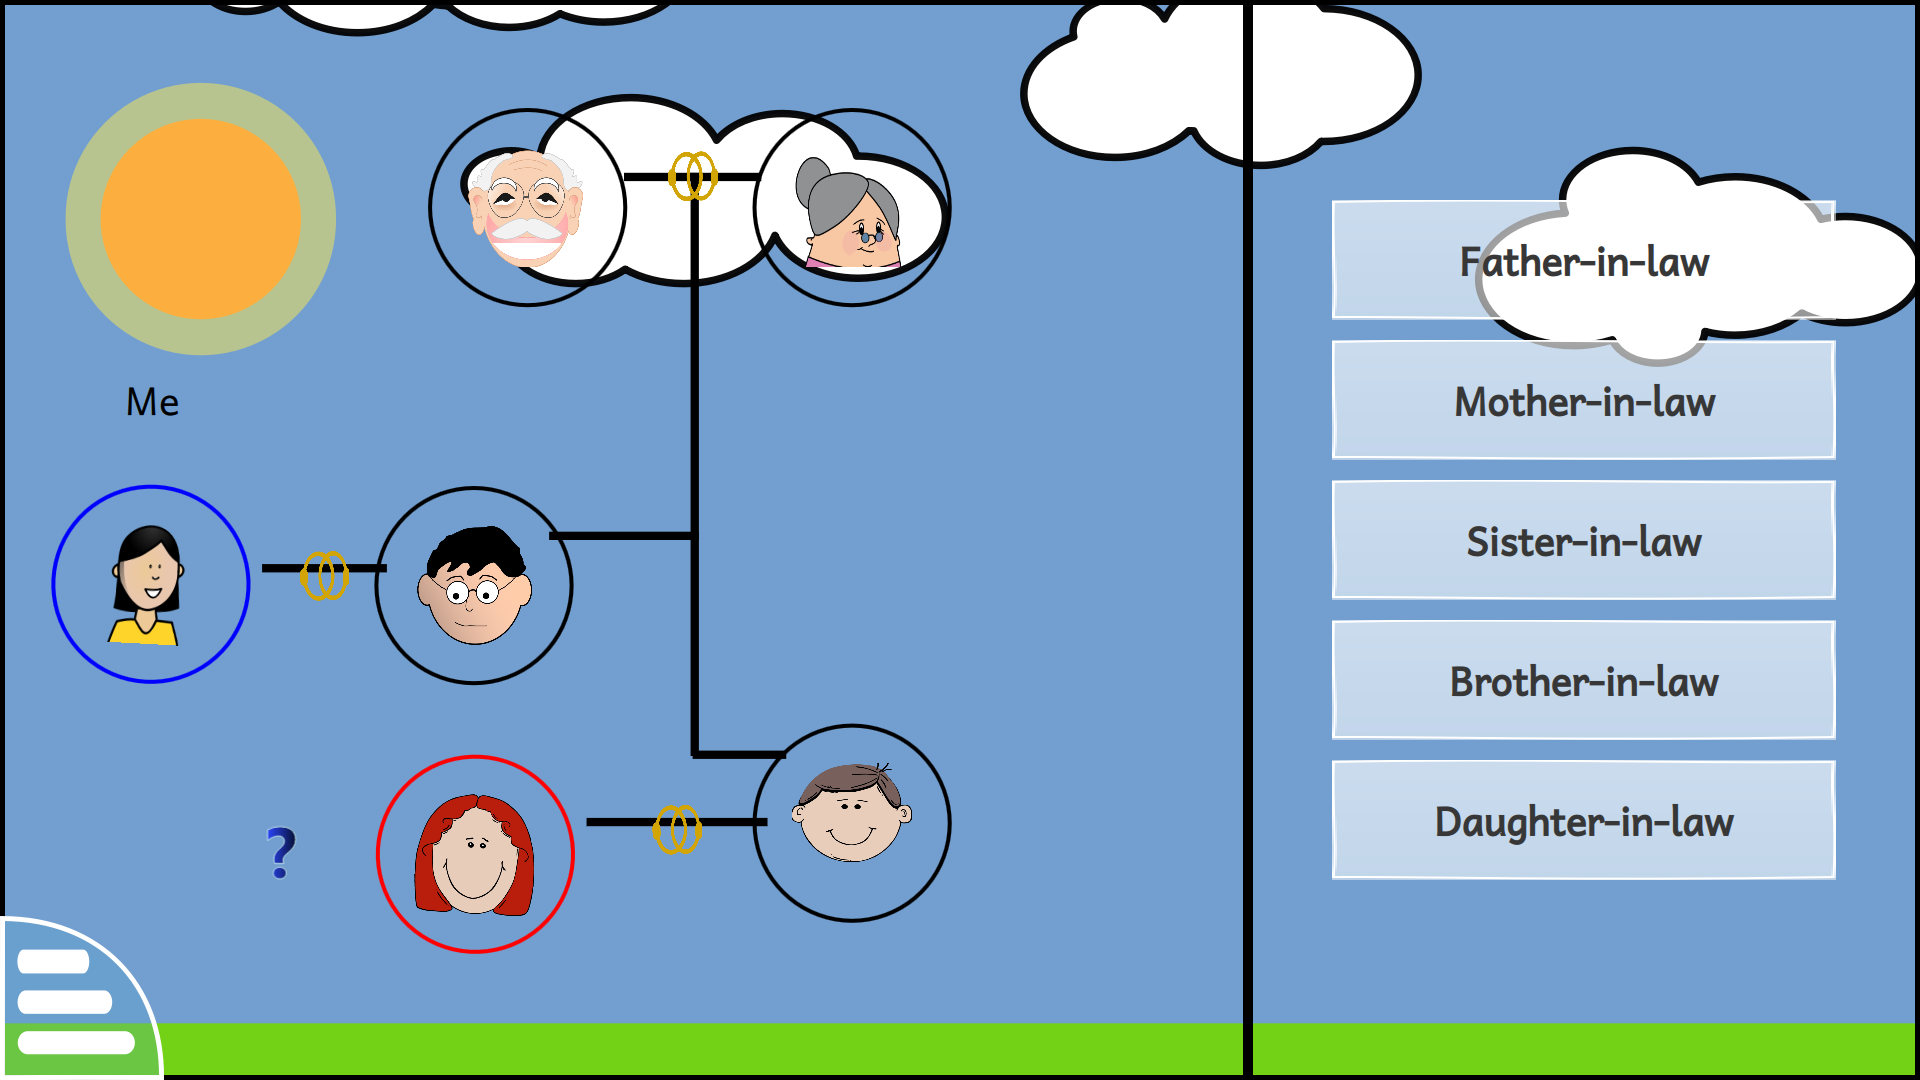
\includegraphics[width=1.0\linewidth]{family}
\caption{Current layout of the Family Activity}
\end{figure}

\begin{figure}[H]
\centering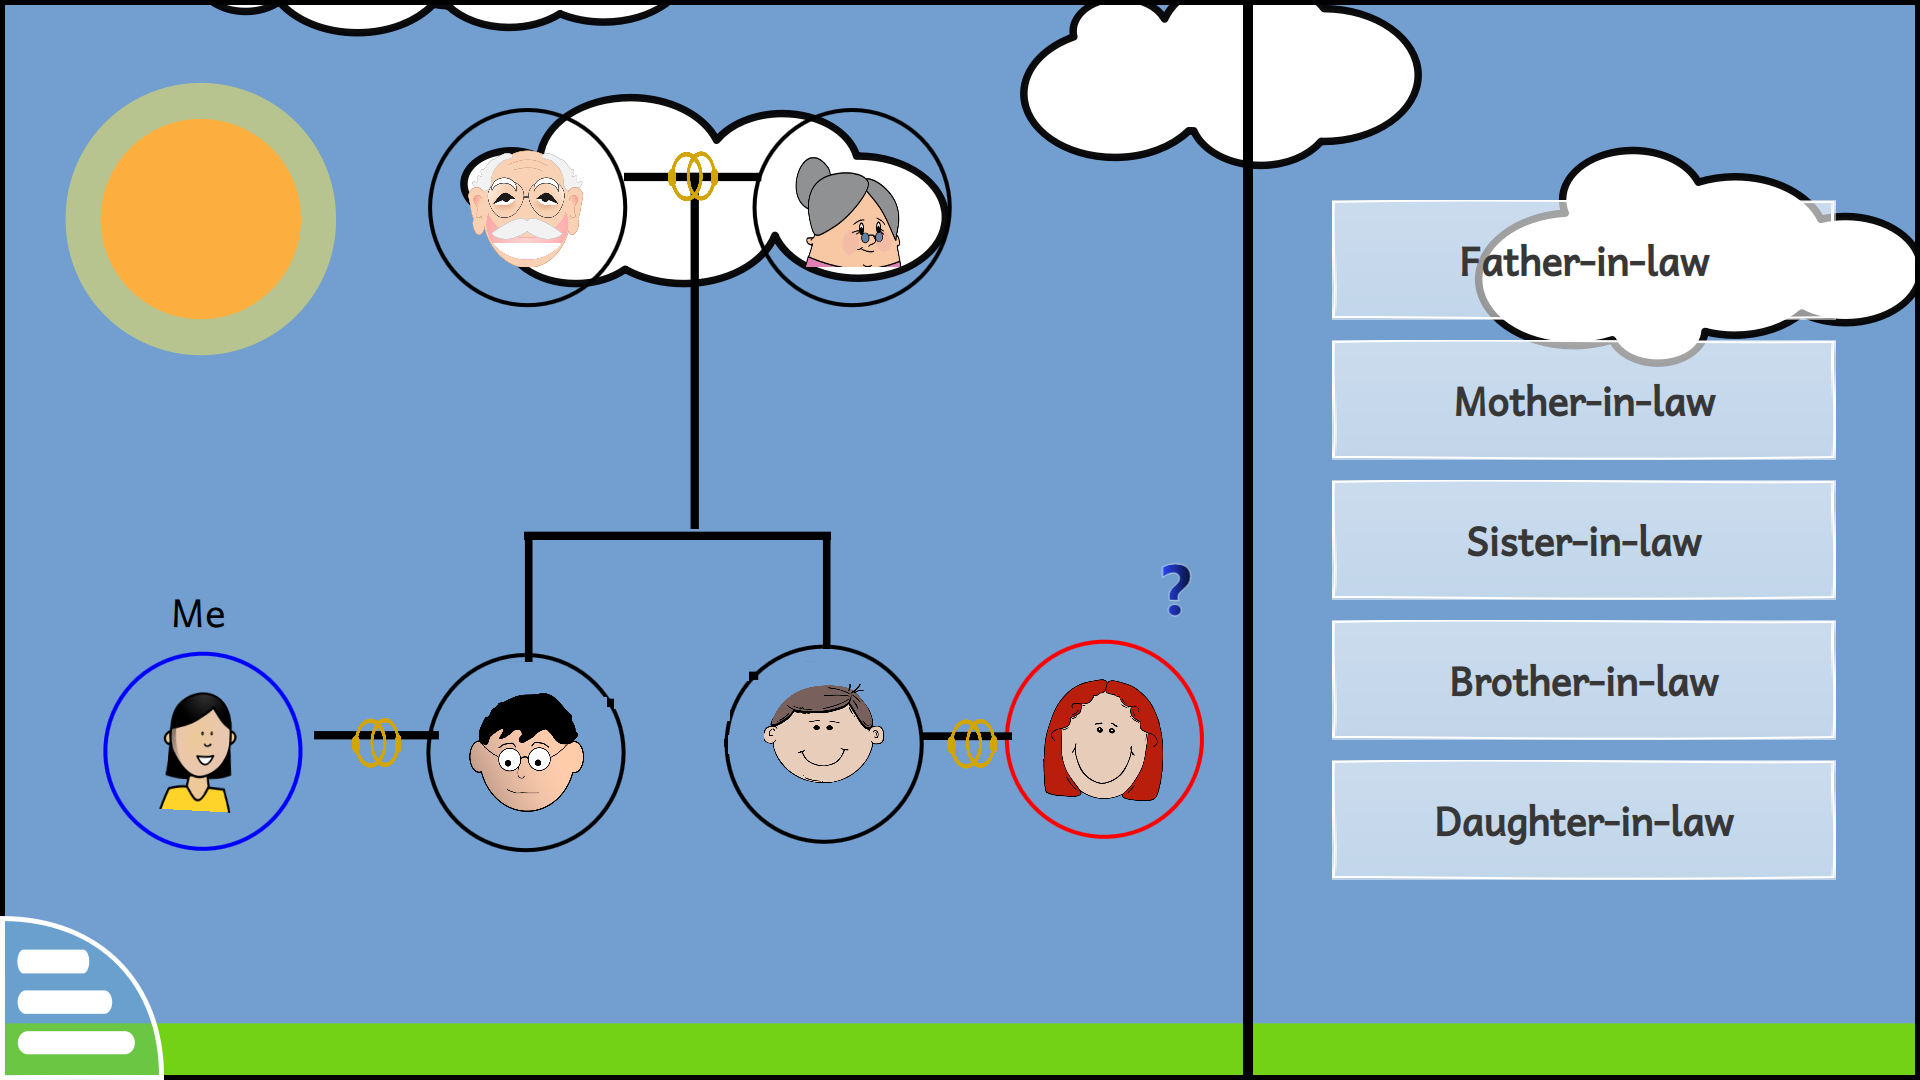
\includegraphics[width=1.0\linewidth]{family_test_2}
\caption{Sketch of the Final layout of the Family Activity}
\end{figure}

\textbf{Extended Goals:}

\begin{itemize}
\item In the existing activity, for a given pair, the user will have to choose the correct relation. There will be one more activity besides the existing activity
\item In the new activity, which will inherit the existing activity, a relation will be provided and the child will have to click on the correct pair which demonstrates the given relation
\end{itemize}



% =======================
% Garbage Recycle
% =======================
%\subsection{Garbage Recycle}

%This activity will be done from scratch as the implementation in the given branch doesn't match with the description. I will be using images from \href{https://openclipart.org/}{openclipart.org} and it will have the following features:

%\begin{itemize}

%\item The activity will begin with a tutorial explaining the basics of different types of recycling procedure for different materials, along with the goal of the activity.

%\item Garbages of different types will be available in the table at the start of each level.

%\item The user will have to put the waste materials in it's correct recycling bin. On placing the waste in it's correct bin, it will be recycled properly. The goal of the activity is to correctly recycle each of the wastes as provided in each levels.

%\item Items will be placed on it's respective bin via drag and drop

%\item With progress of levels, there will be an increase in the categories of waste materials, in order to maintain a proper difficulty curve.

%\end{itemize}

% =======================
% Garbage Recycle
% =======================

\subsection{Digital Electricity}

The core simulation of electricity is done and the circuits are working properly. There exists a \textit{"Free Mode"} where the children can use any component to build a circuit and test it on their own. But to make sure it is easier for the children to understand it, we have to illustrate how each of the components works in a circuit via properly designed levels and instructions. For this project, I propose:

\begin{itemize}
\item There will be levels to teach the children on how to use the components. These levels are broadly divided into three parts:
\begin{itemize}
\item The first part will be a very basic one: the aim will just be to learn how to use the component. For example, if the component is the \textit{Or Gate}, the child will be asked to light the bulb using the "1" and "0" input, or with two "1" inputs.
\begin{figure}[H]
\centering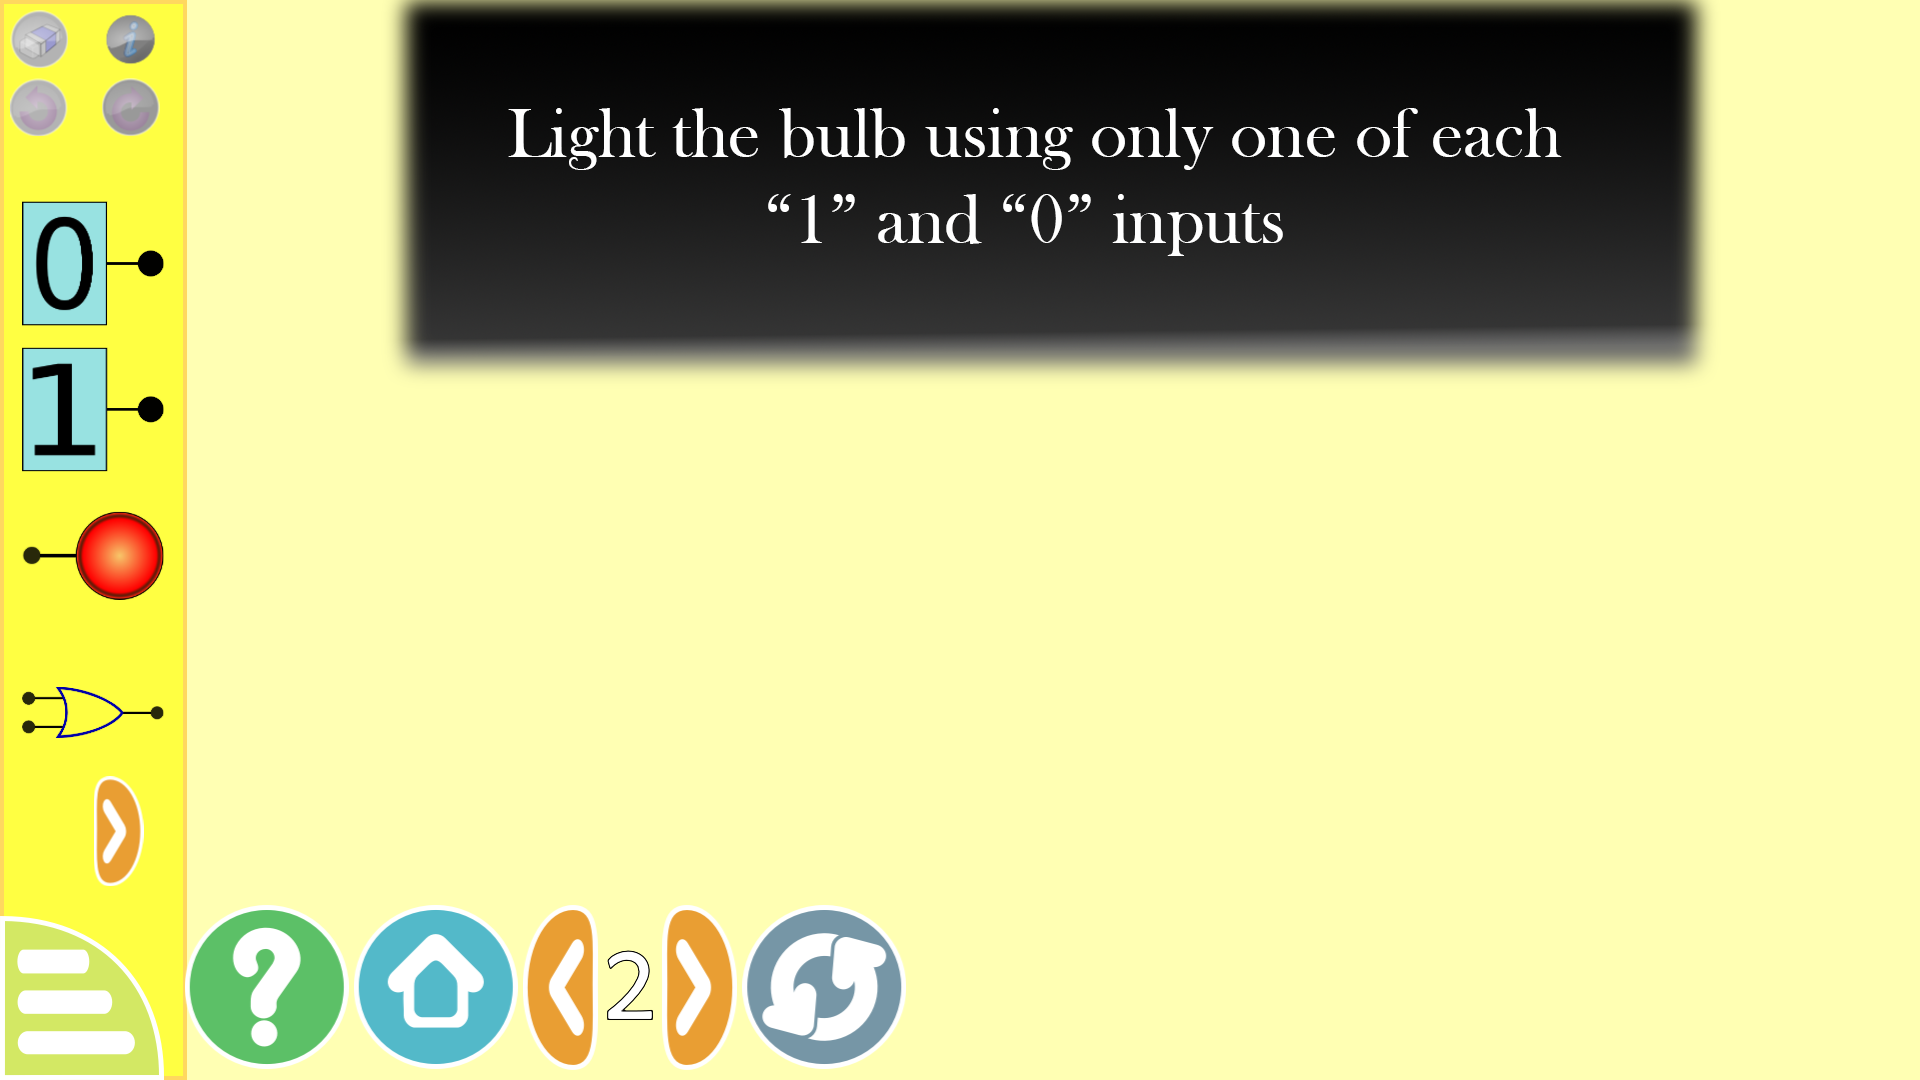
\includegraphics[width=1.0\linewidth]{digital_level_2}
\caption{Digital Electricity: Basics}
\end{figure}
\item The second part will take the previous concepts a bit further and will ask the child to solve a simple problem using the component, maybe reusing it more than once. This will allow the child to get an in-depth understanding on how to use the component and what it’s purpose are. For example, for the \textit{Or Gate}, the child will be asked to light the bulb from three power sources, such that the bulb should be on if at least one of the power sources is turned on
\begin{figure}[H]
\centering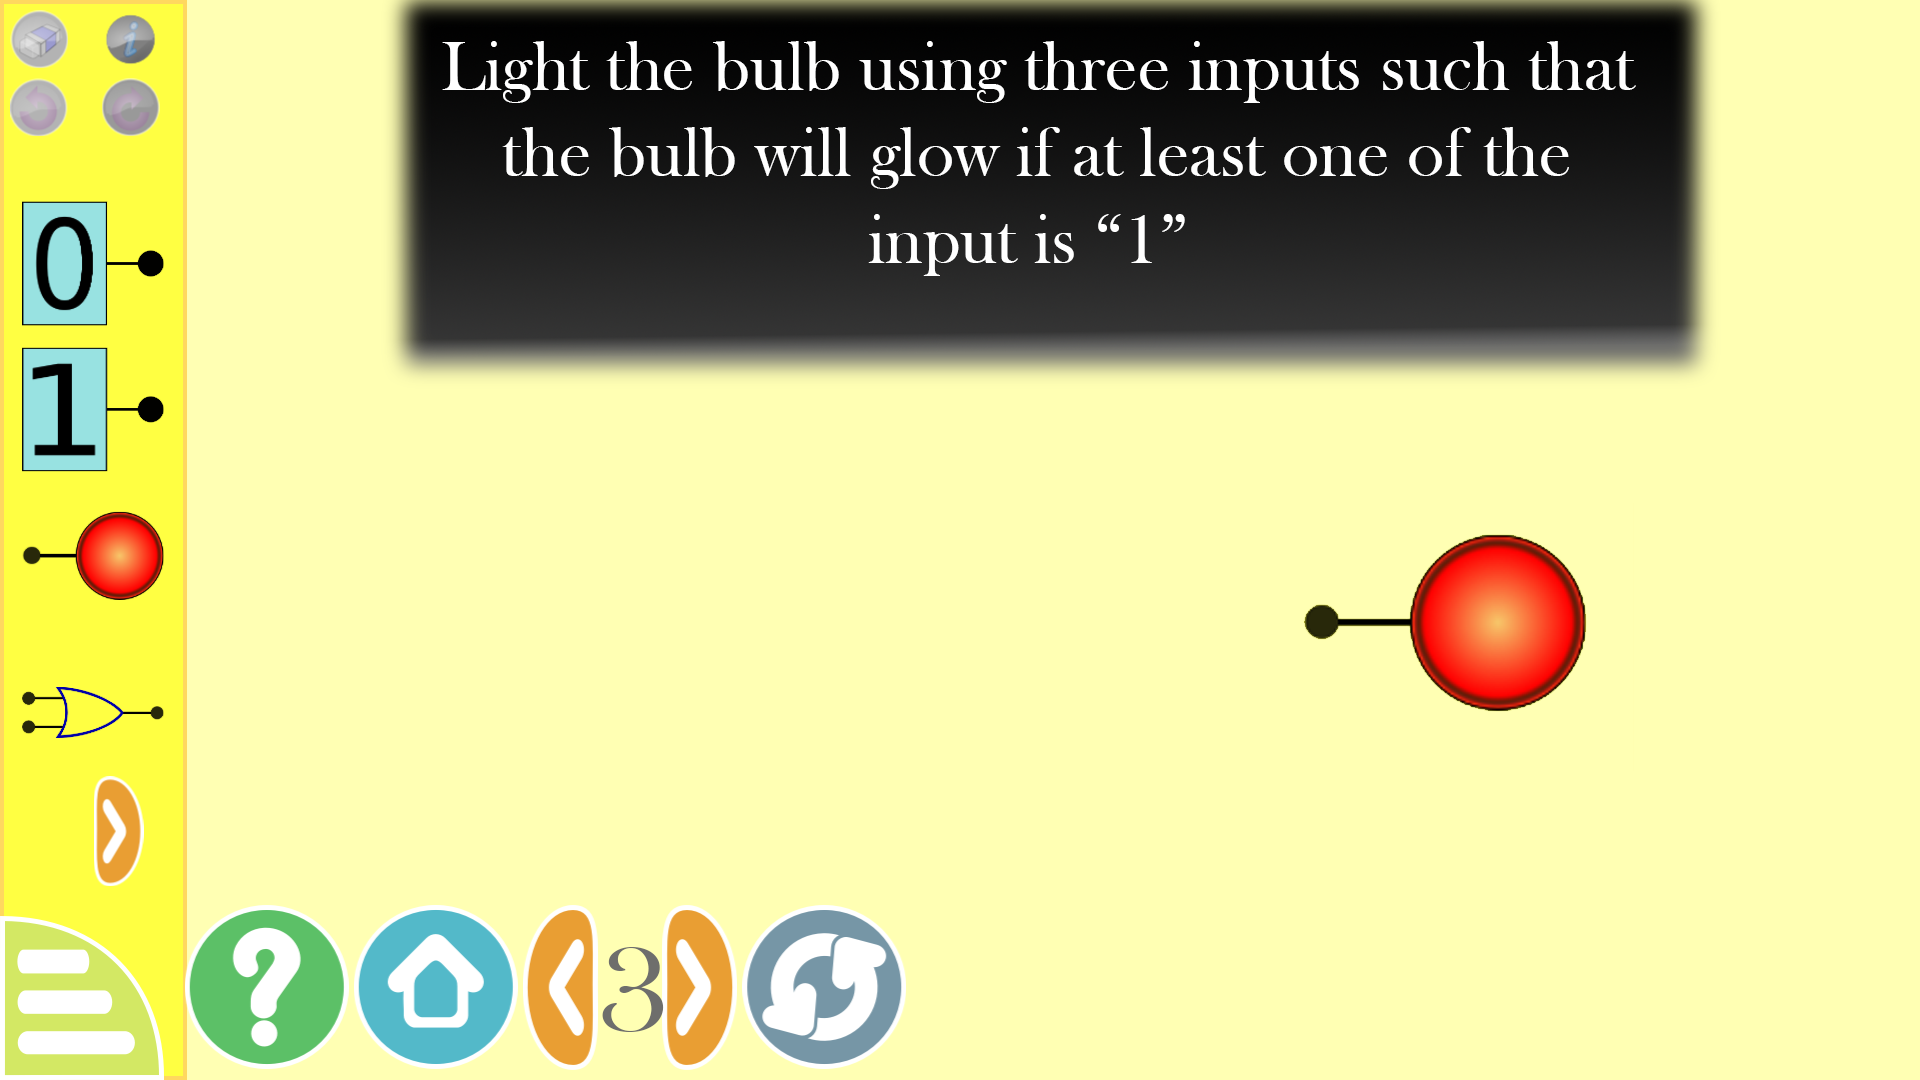
\includegraphics[width=1.0\linewidth]{digital_level_3}
\caption{Digital Electricity: Second Step}
\end{figure}
\item The third part will ask the child to complete a given incomplete circuit, making use of the component and the previously learned components. It will ask the child to complete the circuit with limited number of the provided components
\begin{figure}[H]
\centering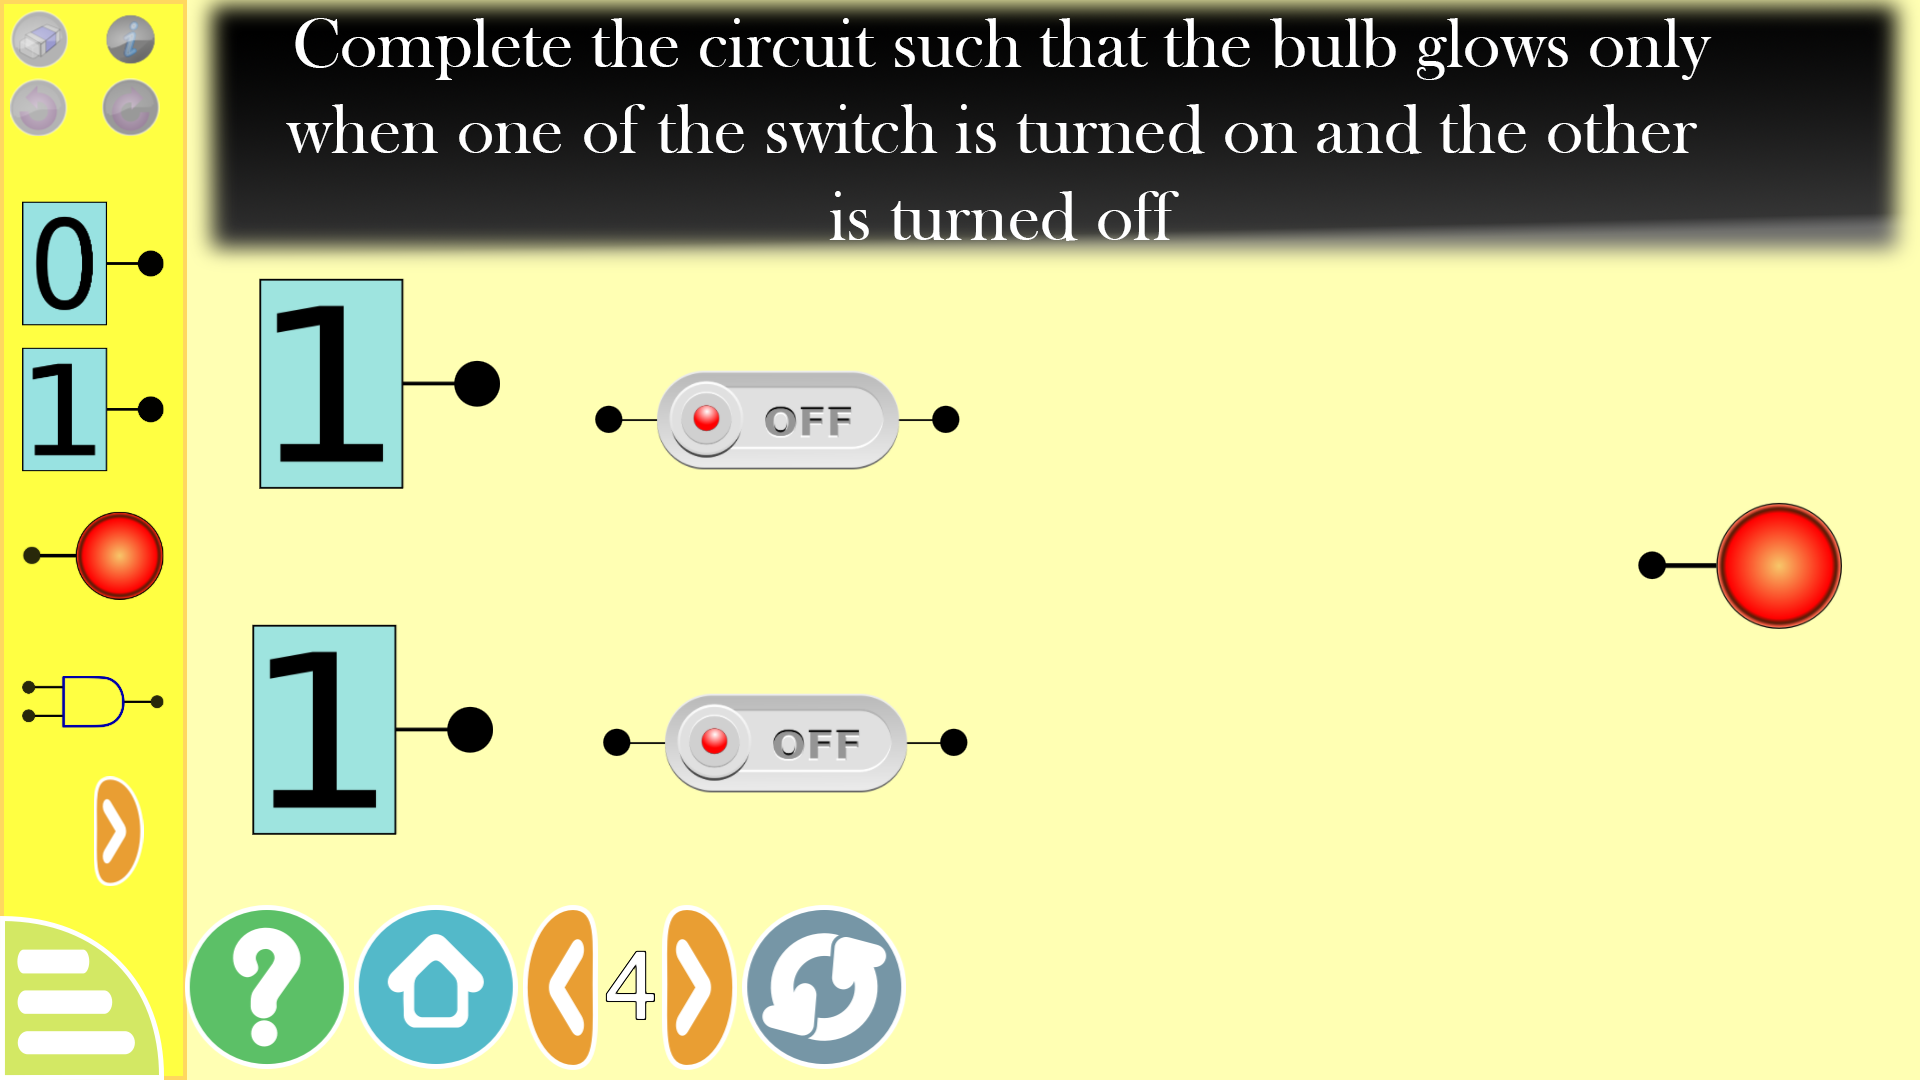
\includegraphics[width=0.9\linewidth]{digital_level_4}
\caption{Digital Electricity: Third Step}
\end{figure}
\end{itemize}
\item The final answers for each of the above levels will be validated using an "ok" button
\item Whenever there is a level where a specific item is used for the first time, there will be an instruction text to inform the children on what the specific component does and how to operate it
\begin{figure}[H]
\centering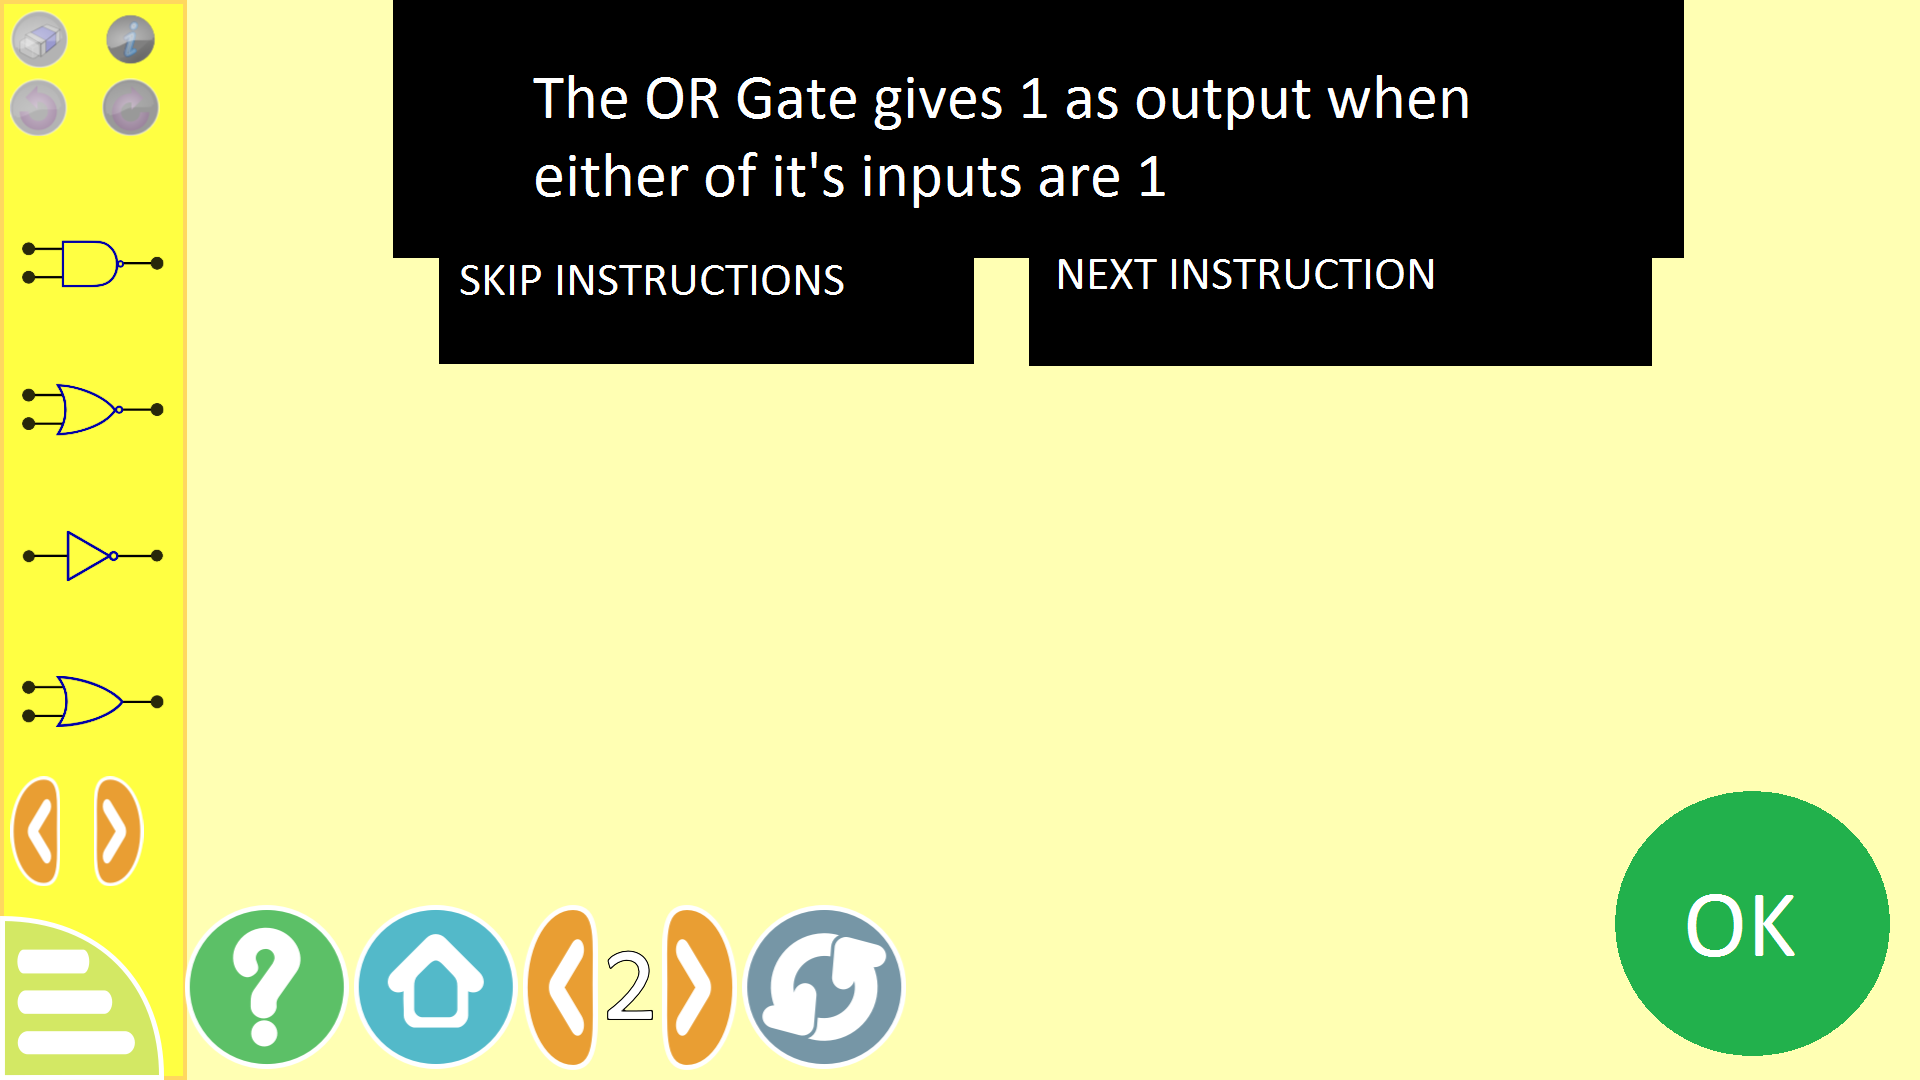
\includegraphics[width=0.9\linewidth]{digital_electricity}
\caption{Digital Electricity: Instructions}
\end{figure}
\item There will be a free mode, as it is present in the current implementation of the activity, where the child can try out any combination of circuits and test it. This “free mode” will be present after the levels are over, once the child has understood the concepts of each and every components and how to use it
\item For small screen devices like tablets and phones, it is uneasy to select the tools ( delete, rotate left, rotate right and info). To improve this, I will be adding them on a ListView, which can be expanded and collapsed when the "\textit{Tools}" option is clicked. (Demo: \href{https://youtu.be/l3ShC4ghRWE}{https://youtu.be/l3ShC4ghRWE})
\item Since the basic simulation is already done in the current progress of the activity, I can directly move on to the coding part, implementing the different levels for the activity
\end{itemize}


%\subsection{ \textbf{Additional Task}: Object Arrangement}

%This activity will be created from scratch, in order to expand the current ordering activity to a more generic version of it. It will have the following features:

%\begin{itemize}

%\item I will be using \href{https://openclipart.org/}{openclipart.org} and Inkscape for the images

%\item Different types of objects will be provided at the start of each levels and the user will be asked to arrange them in a specific order (ascending or descending) based on a given parameter (height or weight)

%\item A toolbox will be provided to the user with the help of which the user can measure the required property of an item

%\item The measured properties will be marked on the object. If a property of an object is not yet measured, it will be marked as unknown.

%\item With the proper measurements, the user will then arrange the items in the correct order of the parameter

%\end{itemize}

%\begin{figure}[H]
%\centering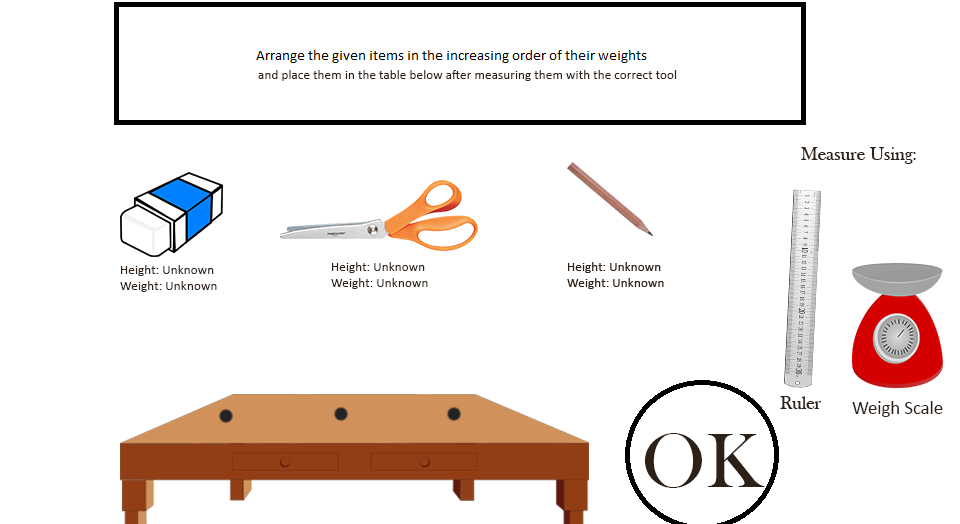
\includegraphics[width=1.0\linewidth]{arrangement}
%\caption{Object Arrangement}
%\end{figure}

%/*2d matrix, Tux, door and few pickups. command tux to take all pickups and move out of the door. Commands - rotate (+-90, +180), move forward (x blocks)*/

%/*Physics*/

%/*Complete incomplete activities*/

% Garbage, ordering, Solar system, family

\section{Timeline}
\label{S:1}

\textbf{May 5, 2017 - May 30, 2017: Community Bonding Period}

\begin{itemize}
\item I will interact and consult with my mentors.
\item I will take an in-depth look at the implementation of the activities in my proposal, discussing about the same with my mentors, so as to devise an optimum method to implement the proposed tasks.
\item I will look up the documentations and learn about box2d, the physics engine I will be using for the submarine activity
\item I will look for the necessary resources (images and audio clips) required for my proposed projects.
\end{itemize}

\textbf{May 31, 2017 - July 10, 2017: \textit{Pilot a Submarine}}

\begin{itemize}

\item \textbf{May 31 - June 5: \textit{Basic Structure, Instructions}}

\begin{itemize}
\item Implement the basic layout of the activity, which includes the submarine itself, the surrounding environment, the gates, the colliders such as the rocks and ships. Also, include the basic components of the submarine: the engine, rudders and air tanks.

\item Create tutorials for the activity: explaining the use of the components of the submarine (engine, rudders and the air tanks) and the goal of the activity.

\end{itemize}

\textbf{Milestone to be reviewed}
\begin{itemize}
\item Review the basic layout and the tutorials of the activity
\end{itemize}

\item \textbf{June 6 - June 20: \textit{Movement, Physics, Collisions and animations}}

\begin{itemize}
\item Implement basic movement of the submarine, physics and collision handling of the submarine using box2d
\item Detect pickups, game over and succesful level completion
\item Implement animations of submarine
\end{itemize}

\textbf{Milestone to be reviewed}
\begin{itemize}
\item The movement, controls, physics, collisions and animations. Changes will be made if necessary
\end{itemize}

\item \textbf{June 21 - June 30: \textit{Implement levels with difficulty}}
\begin{itemize}
\item Implement different levels while maintaining a proper difficulty curve as mentioned in the “Implementation Details”
\end{itemize}

\textbf{Milestone to be reviewed}
\begin{itemize}
\item Review the levels and their difficulty. Changes will be made if necessary to create a proper balance in the difficulty in the levels
\end{itemize}

\item \textbf{July 1 - July 10: \textit{Testing and bug fixing}}
\begin{itemize}
\item Test the activity on various platforms and screen sizes
\item Get reviews for the overall activity from my mentors
\item Make necessary changes based on the reviews from my mentors
\end{itemize}

\end{itemize}

\textbf{July 11, 2017 - July 31, 2017: \textit{Family}}
\begin{itemize}

\item \textbf{July 11 - July 18: \textit{Improve layouts}}
\begin{itemize}
\item Change the layout of the activity to make sure that the implementation is clean and doesn't override other components of the activity
\end{itemize}

\textbf{Milestone to be reviewed}
\begin{itemize}
\item Review the layout of the activity and make changes if necessary
\end{itemize}

\item \textbf{July 19 - July 25: \textit{Implement the parallel activity}}
\begin{itemize}
\item Implement the parallel activity: given a relation, the user will have to click on a pair which satisfies the given relation
\end{itemize}

\textbf{Milestone to be reviewed}
\begin{itemize}
\item Review the new activity from my mentors and make necessary changes
\end{itemize}

\item \textbf{July 26 - July 31: \textit{Testing}}
\begin{itemize}
\item Test the activity on various platforms and screen sizes
\item Rigorous testing of the overall activity for various corner cases which may break the workflow of the activity, analysing and fixing the bugs
\item Get reviews for the overall activity from my mentor
\item Make the necessary changes based on the reviews from my mentors
\end{itemize}

\end{itemize}

\textbf{August 1, 2017 - August 29, 2017: \textit{Digital Electricity}}

\begin{itemize}

\item \textbf{August 1 - August 5: \textit{Initial levels, Instructions}}

\begin{itemize}
\item Fix tools icon being too small for devices with small screen size by implementing the expandable and collapsible ListView
\item Create the initial tutorial levels which are aimed at teaching the basic workings of the components
\item Display the instructions at the beginning of the levels where a new component is used for the first time
\end{itemize}

\textbf{Milestone to be reviewed}
\begin{itemize}
\item Review the initial levels, tutorials and instructions and make the necessary changes to make the concepts easier to understand for newcomers
\end{itemize}

\item \textbf{August 6 - August 17: \textit{Implement levels with difficulty}}

\begin{itemize}
\item Provide a specific problem to the user and ask them to solve it using only specific number of components
\item Implement restricting the number of components that can be used per level to that specified in the level
\item Checking the resultant circuit arrangement after the \textit{"ok"} button is clicked, and display the result to the user.
\item Move the existing “free mode” in the end as the last level, when all the previous level are completed by the user
\end{itemize}

\textbf{Milestone to be reviewed}
\begin{itemize}
\item Review the levels and it’s difficulty and make changes if necessary to adjust the difficulty of the levels
\end{itemize}

\item \textbf{August 18 - August 21: \textit{Testing}}

\begin{itemize}
\item Testing the activity on various platforms and screen sizes
\item Rigorous testing of the overall activity for various corner cases which may break the workflow of the activity, analysing and fixing the bugs
\end{itemize}

\textbf{Milestone to be reviewed}
\begin{itemize}
\item Review of the overall activity, especially on various devices and screen sizes
\end{itemize}

\item \textbf{August 22 - August 29: \textit{Review}}

\begin{itemize}
\item Get reviews from my mentors on the overall activity
\item Make necessary changes based on the reviews
\item Submit the code for final evaluation
\end{itemize}

\end{itemize}

%\textbf{August 22, 2017 - August 29, 2017: \textit{Final Week}}

%\begin{itemize}
%\item Rigorous testing of the activities on various platforms
%\item Fixing the reported bugs
%\item Submit the code for final evaluation
%\end{itemize}

\textbf{Other commitments}

\begin{itemize}
\item I will be having exams from June 1st to June 15th. During that timeline, I will be able to work ~3 hours per day
\item I might be out of station from July 10th to 16th. I will be able to work in my free time, giving around 6 hours per day
\item During the rest of the period, I will be able to work 8-10 hours per day or 40 hours per week
\end{itemize}

\section{About Me}
\label{S:1}

I am a third year undergraduate engineering student from Maulana Abul Kalam Azad University of Technology ( formerly known as West Bengal University of Technology), pursuing B.Tech in Computer Science and Engineering. I have been contributing to KDE for the past few months on the Qt version of GCompris, which helped me to get familiar with Qt and the overall GCompris codebase.

My contributions on GCompris include:

\begin{itemize}

\item Display the characters attempted by the user in the Hangman activity

\href{https://github.com/gcompris/GCompris-qt/commit/8ab75acf49431c685021f3cd0e58cf31f3fa4568}{https://github.com/gcompris/GCompris-qt/commit/\\8ab75acf49431c685021f3cd0e58cf31f3fa4568}

\item Adding a Directory class in Core to directly get a list of all files in a given directory

\href{https://github.com/gcompris/GCompris-qt/commit/955462b943c34fc130d1a68fcfb0e1ec6393a3f0}{https://github.com/gcompris/GCompris-qt/commit/\\955462b943c34fc130d1a68fcfb0e1ec6393a3f0}

\item Improve the algorithm to add new levels in the categorization activity, so that we do not need to change the code while adding new levels. Also, added odd-even category in the categorization activity

\href{https://github.com/gcompris/GCompris-qt/commit/db7a4a9b743a3521c7c68f0b2b54719cbc9582db}{https://github.com/gcompris/GCompris-qt/commit/\\db7a4a9b743a3521c7c68f0b2b54719cbc9582db}

\item Display a black point in drawletters and drawnumbers activity whenever a line cannot be drawn for a given input

\href{https://github.com/gcompris/GCompris-qt/commit/eaf8dd326dd3f5581995155739be5c72af744f92}{https://github.com/gcompris/GCompris-qt/commit/\\eaf8dd326dd3f5581995155739be5c72af744f92}

\item \textbf{Under review}: Ordering activity, which aims at arranging numbers and alphabets in it's increasing or decreasing order

\href{https://github.com/gcompris/GCompris-qt/pull/172}{https://github.com/gcompris/GCompris-qt/pull/172}

\item \textbf{Under review}: Allow only certain activities to take part in the expert mode of categorization activity

\href{https://github.com/gcompris/GCompris-qt/pull/181}{https://github.com/gcompris/GCompris-qt/pull/181}

\item Added images to the word dataset of gcompris, which is used in the odd-even category of the categorization activity

\href{https://github.com/gcompris/GCompris-words/tree/master/words/numbers}{github.com/gcompris/GCompris-words/tree/master/words/numbers}

\end{itemize}

I am also the head of our college's programming club, where we create awareness about open source and encourage newcomers to take part in open source contribution.

Some of my other open source projects include contributing to Algorithm Visualizer (\href{https://github.com/parkjs814/AlgorithmVisualizer}{github.com/parkjs814/AlgorithmVisualizer}), Battery Manager ( \href{https://github.com/BytesClub/Battery_Manager}{github.com/BytesClub/Battery-Manager} ), Simulator ( \href{https://github.com/BytesClub/Simulator}{github.com/BytesClub/\\Simulator} ) and few video game projects which I build during my free time, namely: Followed (\href{https://github.com/RudraNilBasu/AsylumJam2016}{github.com/RudraNilBasu/\\AsylumJam2016}), Fortior (\href{https://github.com/RudraNilBasu/Fortior}{github.com/RudraNilBasu/Fortior}) and a Quiz game (\href{https://github.com/RudraNilBasu/Quiz-Game}{github.com/RudraNilBasu/Quiz-Game}) to name a few.

All of my open source projects can be found on my Github profile: \href{https://github.com/RudraNilBasu}{github.com/RudraNilBasu}


Besides this, I have actively taken part in online and offline programming competitions, hackathons and have been involved in video game development, taking part in numerous online and offline game jams. I have faired well in a lot of them, grabbing the top 3 spot few times. My projects have also been the runner’s up for NGF Student Game of the Year Award twice.

\textbf{Blog}: \href{http://rudranilbasu.me/blog/}{rudranilbasu.me/blog}\\

\textbf{Contact Information}:

\textbf{Email ID}: rudra.nil.basu.1996@gmail.com

\textbf{Freenode IRC nick}: rudra

%% The Appendices part is started with the command \appendix;
%% appendix sections are then done as normal sections
%% \appendix

%% \section{}
%% \label{}

%% References
%%
%% Following citation commands can be used in the body text:
%% Usage of \cite is as follows:
%%   \cite{key}          ==>>  [#]
%%   \cite[chap. 2]{key} ==>>  [#, chap. 2]
%%   \citet{key}         ==>>  Author [#]

%% References with bibTeX database:

\bibliographystyle{model1-num-names}
\bibliography{sample.bib}

%% Authors are advised to submit their bibtex database files. They are
%% requested to list a bibtex style file in the manuscript if they do
%% not want to use model1-num-names.bst.

%% References without bibTeX database:

% \begin{thebibliography}{00}

%% \bibitem must have the following form:
%%   \bibitem{key}...
%%

% \bibitem{}

% \end{thebibliography}


\end{document}

%%
%% End of file `elsarticle-template-1-num.tex'.
